% 设置 biblatex 额外选项
% \PassOptionsToPackage{gbpub=false, gbtype=false}{biblatex}

% 载入 SJTUThesis 模版
% \documentclass[degree=doctor, zihao=-4, language=english, review]{sjtuthesis}
% \documentclass[degree=master, zihao=-4]{sjtuthesis}
\documentclass[degree=bachelor, language=english, openany, oneside]{sjtuthesis}
% \documentclass[degree=course, language=english, openright, twoside]{sjtuthesis}
% 选项
%   degree=[doctor|master|bachelor|course],     % 必选,学位类型
%   language=[chinese|english],                 % 可选(默认:chinese),论文的主要语言
%   bibstyle=[gb7714-2015|gb7714-2015ay|ieee],  % 可选(默认:gb7714-2015),参考文献样式
%   review,                                     % 可选(默认:关闭),盲审模式

% 所有其它可能用到的包都统一放到这里了,可以根据自己的实际添加或者删除。
\usepackage{sjtuthesis}

% 定义图片文件目录与扩展名
\graphicspath{{figure/}}
\DeclareGraphicsExtensions{.pdf,.eps,.png,.jpg,.jpeg}

% 导入参考文献数据库
\addbibresource{bib/thesis.bib}

% 信息录入,必须在导言区进行!
% !TEX root = ../thesis.tex

%TC:ignore

\title{胆甾液晶的积分方程和密度泛函理论研究}
\author{文\quad{}聪}
\studentid{516111910163}
\supervisor{吴量}
% \assisupervisor{某某教授}
\degree{理学学士}
\major{化学(致远荣誉计划)}
\department{化学化工学院,致远学院}
\coursename{某某课程}
\date{2020年05月10日}
% \fund{国家 973 项目 (No. 2025CB000000) \\ 国家自然科学基金 (No. 81120250000)}
\keywords{液晶,统计力学,密度泛函理论}

\entitle{The Integral Equation and Density Function Theory of Cholesteric Liquids}
\enauthor{Cong Wen}
\ensupervisor{Liang Wu}
% \enassisupervisor{Prof. Uom Uom}
\endegree{Bachelor of Science}
\enmajor{Chemistry (Zhiyuan Honors Program)}
\endepartment{School of Chemistry and Chemical Engineering, Zhiyuan College}
\endate{May. 10th, 2020}
% \enfund{National Basic Research Program of China (Grant No. 2025CB000000) \\
%   National Natural Science Foundation of China (Grant No. 81120250000)}
\enkeywords{Liquid Crystal, Statistical Mechanics, Density Function Theory}

%TC:endignore


% 自定义项目标签名称
% \sjtuSetLabel{
%   listfigure = {图\quad 录},
%   listtable  = {表\quad 录}
% }

\begin{document}

% 无编号内容:中英文论文封面、授权页
\maketitle
\makeDeclareOriginality[pdf/originality.pdf]
\makeDeclareAuthorization

% 使用罗马数字对前言编号
\frontmatter

% 摘要
% !TEX root = ../thesis.tex

\begin{abstract}
	对于一类特殊的分子,在计算机分子模拟中观察到了其胆甾相(手性向列向),但整个计算过程仍然非常耗时,所以我们构建了一个可以更加便捷地预测这类分子热力学性质的理论框架。理论体系以Onsager的液晶相变理论为基础,以Parsons-Lee的硬球近似方法为改进,我们可以用密度泛函理论(DFT)计算出这类分子的径向分布函数(ODF)。为了预测其胆甾相,我们进一步使用Straley的近似方法,以向列相的ODF近似为胆甾相的局部ODF,从而可以预测得到液晶分子在胆甾相下的热力学性质。
\end{abstract}

\begin{enabstract}
  Cholesteric phase is found for certain liquid crystals molecules in computer simulation, but the process is still very time-consuming, so we constructed a theoretical framework to predict the thermodynamic properties of this molecule. Based on Onsager’s theory and Parsons-Lee’s improvement of phase transition of liquid crystals, we used density function theory to calculate the orientational distribution function of the molecule. And in addition, by applying Straley’s approximation method, we calculated the cholesteric pitches for a given density. We thus found a way to predict the thermodynamic properties of cholesteric liquid crystals.
\end{enabstract}


% 目录、插图目录、表格目录
\tableofcontents
\listoffigures
\listoftables
\listofalgorithms

% 主要符号、缩略词对照表
% !TEX root = ../thesis.tex

%TC:ignore

\begin{nomenclature}{rl}
\label{chap:symb}
  $\epsilon_0$ & Energy Unit \\
  $k$ & Boltzmann Constant \\
  $T$ & Temperature \\
  $\beta$ & $\frac{1}{kT}$ \\
  $O$ & Ensemble Average of a Physical Property \\
  $O^*$ & Reduced Ensemble Average of a Physical Property \\
  $F$ & Free Energy \\
  $P$ & Pressure \\
  $\mu$ & Chemical Potential \\
  $p$ & Cholesteric Pitch \\
  $q$ & $2\pi/p$, Cholesteric Pitch Wave Vector \\
  $f(\vec{u})$ & Orientational Distribution Function(ODF) \\
  $v_m$ & Molecular Volume \\
  $\rho$ & Number Density \\
  $\eta$ & $\rho v_m$, Packing Fraction\\
\end{nomenclature}

%TC:endignore


% 使用阿拉伯数字对正文编号
\mainmatter

% 论文正文
% !TEX root = ../thesis.tex

\chapter{Introduction}


This undergraduate thesis mainly investigated electrically neutral lyotropic liquid crystals, this is a kind of typical soft matter. Historically, liquid crystals were discovered in 1888 when the Australian botanist Friedrich Reinitzer studied cholesterol benzoate, which is now known as cholesteric liquid crystals, and his friend German physicist Otto Lehmann named it "Liquid Crystal".

Microscopically, liquid crystals are mostly rod-like molecules, which enables them to behave anisotropically under certain circumstances. Under high temperature (so that the kinetic energy dominates) or very low density, molecules can still move freely regardless of its rod-like shape, and they behaves just like normal fluids, this is the isotropic phase. But it can be imagined that under high density or low temperature (so that the interaction between molecules will dominate over kinetic energy), molecules are pushing each other and tend to lean on each other in a near parallel way, so they will be oriented preferably in a certain direction, this is the nematic phase. And further if they are more than rod-like, having chiral mutual interactions between each other, they further tend to lean on each other with a preferable non zero angle, behaves periodically in the space, this is the cholesteric phase.

But the understanding of liquid crystal at a molecular level is still challenging, in a preceding work by Liang\cite{Liang2017SM}, a coarse-grained molecular model is developed and represented by flexible chain with helical interactions (FCh). This is a reasonable approximation to a number of ordinary cholesteric liquid crystals, such as double strand DNA. Both nematic phase and cholesteric phase was observed by molecular dynamics (MD) simulation FCh molecules.

To further investigate how the phase transition happens and provide insight into the relationship between microscopic molecular characteristics and the macroscopic phase behavior, a theoretical method is developed in this thesis to give a prediction of thermodynamic properties of FCh model. The theory is based on Onsager's original theory\cite{Onsager1949NYAS} of phase transition of liquid crystals, and makes use of DFT method to give a depiction of the thermodynamic properties of the phase transition of FCh. In addition, a modular program is developed from scratch for the phase diagram computation of a wide range of liquid crystal molecules including FCh.


% !TeX root = ../thesis.tex

\chapter{Molecular Model}
The molecular model is given in Fig. \ref{fig:fch}

\begin{figure}[h!]
 	\centering
 	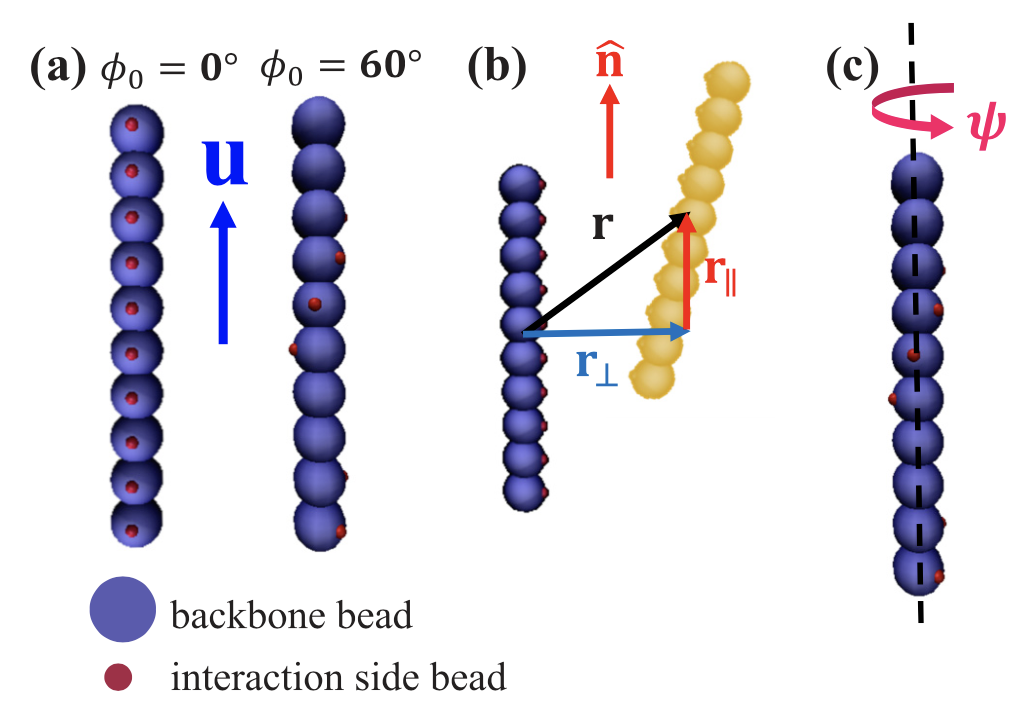
\includegraphics[width=\linewidth]{fch.png} \\
	\caption[Schematic of FCh model]{Schematic figure of FCh model\cite{Liang2019PRE}}
	\label{fig:fch}
\end{figure}

\section{Flexible Chain with Helical Interactions (FCh)}

\section{Existing Simulation Results}

\section{Summary}


% !TeX root = ../thesis.tex
\newcommand{\mat}[1]{\left(\begin{matrix}#1\end{matrix}\right)}
\newcommand{\arr}[2][n]{#2_1,#2_2,\cdots,#2_{#1}}
\newcommand{\xsim}[1]{\stackrel{#1}{\sim}}
\newcommand{\iprod}[2]{\langle#1,#2\rangle}
\newcommand{\mbb}[1]{\mathbb{#1}}
\newcommand{\mbf}[1]{\mathbf{#1}}
\newcommand{\mcal}[1]{\mathcal{#1}}
\newcommand{\mfk}[1]{\mathfrak{#1}}
\newcommand{\mrm}[1]{\mathrm{#1}}
\newcommand{\mcr}[1]{\mathscr{#1}}
\newcommand{\on}[1]{\operatorname{#1}}
\newcommand{\ol}[1]{\overline{#1}}
\newcommand{\wt}[1]{\widetilde{#1}}
\newcommand{\mr}[1]{\mathring{#1}}
\newcommand{\lr}[1]{\langle{#1}\rangle}
\newcommand{\red}[1]{\textcolor{red}{#1}}
\newcommand{\blue}[1]{\textcolor{blue}{#1}}
\newcommand{\green}[1]{\textcolor{green}{#1}}
\newcommand{\tbf}[1]{\textbf{#1}}
\newcommand{\tit}[1]{\textit{#1}}

\chapter{Theoretical Framework}

\section{Statistical Mechanics}
All the topics covered in this thesis are restricted to \textbf{equilibrium statistical mechanics}.

\subsection{Ensemble Theory}
In this part, we will do our best to provide a self-contained introduction of the fundamental knowledge of ensemble theory , which is at the core of statistical mechanics. Readers who are familiar with the derivation are free to skip to the Sec. \ref{SM-ToE-Sum} to read a summary. And we recommend those who are not satisfied to read textbooks[REF of SM].

\subsubsection{Systems and Ensembles}
We define a \textbf{microstate}(replica) of a system to be a specific state in which the mechanical information of every particle is determined. And we define a \textbf{macrostate}(ensemble) of a system to be a probability distribution of all possible microstates. To identify a microstate, you have to designate all the velocities and position of each particles involved, while to identify a macrostate, you only need much fewer physical quantities.

For example, there is a cup of water on the table. This, overall, is a macrostate, and for example, temperature is enough to capture enough information of all water molecules (their averaged kinetic energy). But if you take a magical photo which can record the kinetic information of every molecule, the information contained in the photo is then a microstate, and you need a bunch of variables to identify it, in the magnitude of at least $10^{23}$.

Below we can assume that microstates are discrete, and all the infinite summation are assumed to be convergent.

An ensemble is a working conception of macrostate, it determines a macrostate, and it contains a collection of replicas, each of which represents a microstate, together with a probability distribution.

As for a system, there are three crucial parameters: total energy $E$, number of particles $N$ and volume of the system $V$. For different systems, we have different corresponding ensembles. The most important ones are micro-canonical ensemble, canonical ensemble and grand-canonical ensemble. We next dive into them one by one.

\subsubsection{Isolated system}
An isolated system is a thermodynamic system which does not exchange energy, particles and volume with the environment, i.e. it has fixed $E,V,N$. And the corresponding ensemble is called micro-canonical ensemble.

As a pioneer of statistical mechanics, Boltzmann proposed the posulate of \textit{a prior} probability: For an isolated system with given $(E,V,N)$, the system can be found with equal probability in any microstate.

Now assume the total number of all possible microstates is $\Omega(E,V,N)$, this is the micro-canonical partition function. Then for any given state $s$, we have
\begin{equation}
	p_{mc}(s) = \frac{1}{\Omega(E,V,N)}.
\end{equation}

In any ensemble, the Gibbs entropy is defined as
\begin{equation}
	S=-k\sum_s p(s)\ln p(s),
\end{equation}
in which $s$ is taken over all possible microstates according to the requirement of the system.

\red{HERE to DO maybe}
By using the postulate of equal \textit{a prior} probability, we can derive the condition of three important equilibriums: thermodynamic equilibrium, mechanical equilibrium and chemical equilibrium, which corresponds to equal temperature, pressure and chemical potential.
\red{HERE to DO maybe}

\subsubsection{Closed system}
A closed system is a thermodynamic system which may only exchange energy with the environment. The corresponding ensemble is then called canonical ensemble. Since it is in equilibrium with the environment, although its energy $E$ may vary, it must has a fixed temperature $T$ according to the equilibrium condition.

The probability of a given state $s$ is proportional to $e^{-\beta E_s}$(Boltzmann distribution \red{which can be derived from previous}), then by normalization we get the expression of canonical partition function and the canonical distribution.
\begin{equation}
	Z(T,V,N)=\sum_se^{-\beta E_s}, p_c(s) = \frac{e^{-\beta E_s}}{Z(T,V,N)}
\end{equation}
By splitting the summation $\sum_s$ to $\sum_E\sum_{s, E_s=E}$, we get the relation between canonical partition function and micro-canonical partition function:
\begin{equation}
	Z(T,V,N) = \sum_s e^{-\beta E_s} =\sum_E \Omega(E,V,N)e^{-\beta E}.
\end{equation}

By definition of Gibbs entropy, we know
\begin{equation}
	S=k\ln Z + E/T,
\end{equation}
hence $-kT\ln Z(T,V,N) =E-TS= F(T,V,N)$, this is the Helmholtz free energy. From its differential form
\begin{equation}
	\on{d}F = -S\on{d}T-P\on{d}V+\mu\on{d}N,
\end{equation}
we know the other physical properties expressed from the partition function
\begin{equation}
	S=-\frac{\partial F}{\partial T}, P=-\frac{\partial F}{\partial V}, \mu = \frac{\partial F}{\partial N}.
\end{equation}

\subsubsection{Open system}
An open system is a thermodynamic system which may exchange both energy and particles with the environment. The corresponding ensemble is then called grand-canonical ensemble. Although its energy $E$ and number of particles $N$ may vary, it must has a fixed temperature $T$ and chemical potential $\mu$.

By the similar argument, the probability of a given state $s$ is proportional to $e^{-\beta(E_s-\mu N_s)}$, then by normalization we get the expression of grand-canonical partition function and the grand-canonical distribution.
\begin{equation}
	\Xi(T,V,\mu)=\sum_se^{-\beta (E_s-\mu N_s)}, p_{gc}(s) = \frac{e^{-\beta (E_s-\mu N_s)}}{\Xi(T,V,\mu)}
\end{equation}

By splitting  the summation $\sum_s$ to $\sum_N\sum_{s, N_s=N}$, we get the relation between grand-canonical partition function and canonical partition function:
\begin{equation}
	\Xi(T,V,\mu) = \sum_s e^{-\beta (E_s-\mu N_s)} =\sum_N Z(T,V,N)e^{\beta \mu N}.
\end{equation}
Now the grand potential is defined as $\Phi(T,V,\mu)=-k\ln\Xi(T,V,\mu)$, since
\begin{equation}
	\ln p_{gc}(s) = -\ln\Xi - \beta (E_s - \mu N_s)
\end{equation}
by taking the ensemble average, we get
\begin{equation}
	-S = k\lr{\ln p_{gc}(s)} = -\ln\Xi - \lr{E-\mu N}/T
\end{equation}
Hence we have
\begin{equation}\label{Eqn:GrandPot}
	\Phi(T,V,\mu) = E - TS - \mu N
\end{equation}

Next we derive physical properties from the partition function, from Eqn. \ref{Eqn:GrandPot}, we know
\begin{equation}
	\on{d}\Phi = -S\on{d}T - P\on{d}V- N\on{d}\mu,
\end{equation}
so we have
\begin{equation}
	S=-\frac{\partial\Phi}{\partial T}, P = -\frac{\partial\Phi}{\partial V}, N = -\frac{\partial\Phi}{\partial\mu}
\end{equation}


In addition, since $E,S,V,N$ are all extensive quantities, we know $E(S,V,N)$ is homogeneous with respect to $S,V,N$, then according to Euler's relation, we have
\begin{equation}
	\frac{\partial E}{\partial S}S+\frac{\partial E}{\partial V}V+\frac{\partial E}{\partial N}N=E=TS-PV+\mu N,
\end{equation}
this is called the Gibbs-Duhem relation.

\subsubsection{Minimal Free Energy Principle}
In fact, in equilibrium statistical mechanics, we have several equivalent principles (postulates), we list them here without reasoning, because the readers should be familiar with all of this at their first course of thermodynamics.

\paragraph{Postulate of Equal \textit{a prior} probability}
For an isolated system with given $(E,V,N)$, the system can be found with equal probability in any microstate.
\paragraph{principle of Maximal Entropy}
For an isolated system, the Gibbs entropy reaches its maximal at its equilibrium state.
\paragraph{principle of Minimal Free Energy}
For a closed system, the Helmholtz free energy reaches its minimal at its equilibrium state.
\paragraph{principle of Maximum Work}
For a closed system, the maximal work which the system is capable to do to the environment in a given process is the change in Helmholtz free energy.

\subsubsection{Summary}\label{SM-ToE-Sum}
Tab. \ref{tab:ensemble} is a summary of three most common ensembles, and we give below the formulas to derive other physical properties in case of canonical system and grand-canonical system.

\begin{table}[!h]
	\caption{Summary of Ensembles}
	\label{tab:ensemble}
	\centering
	\begin{tabular}{ccccc}
		\toprule
		System & Condition & Ensemble & Partition Function & Probability $p(s)$\\
		\midrule
		Isolated system & $E,N,V$ fixed & micro-canonical & $\Omega(E,V,N)$ & $\dfrac{1}{\Omega(E,V,N)}$\\
		Closed system & $N,V$ fixed & canonical & $Z(T,V,N)$ & $\dfrac{e^{-\beta E_s} }{Z(T,V,N)}$\\
		Open system & $V$ fixed & grand-canonical & $\Xi(T,V,\mu)$&$\dfrac{e^{-\beta(E_s-\mu N_s)} }{ \Xi(T,V,\mu)}$\\
		\bottomrule
	\end{tabular}
\end{table}

The relations between partition function
\begin{equation*}
	\begin{split}
		Z(T,V,N) = \sum_s e^{-\beta E_s} =\sum_E \Omega(E,V,N)e^{-\beta E},\\
		\Xi(T,V,\mu) = \sum_s e^{-\beta (E_s  - \mu N_s)} = \sum_N Z(T,V,N)e^{\beta N\mu}.
	\end{split}
\end{equation*}


Now we give how physical properties can be computed from the partition function.

In the canonical ensemble, we have
\begin{equation}
	\begin{split}
		F(T,V,N) = -\frac{1}{\beta}\ln Z(T,V,N) = E-TS,\\
	S=-\frac{\partial F}{\partial T}, P=-\frac{\partial F}{\partial V}, \mu = \frac{\partial F}{\partial N}.
	\end{split}
\end{equation}

In the grand-canonical ensemble, we have
\begin{equation}
	\begin{split}
		\Phi(T,V,\mu) = -\frac{1}{\beta}\ln\Xi(T,V,\mu) = -PV,\\
		S=-\frac{\partial\Phi}{\partial T}, P = -\frac{\partial\Phi}{\partial V}, N = -\frac{\partial\Phi}{\partial\mu}.
	\end{split}
\end{equation}

\subsubsection{Ideal Gases}
This part will contain the concrete calculation of partition function of a system, in particular, ideal gas.

In a classical system, the space is continuous, hence the summation $\sum_s$ becomes the integration in phase space $\int\prod\on{d}p_i\on{d}q_i$, in which $p$ and $q$ are all $3$-dimensional vector, and $i$ is taken over all $N$ particles. The canonical partition function then reads
\begin{equation}
	Z(T,V,N) = \frac{1}{h^{3N}N!}\int \prod_i\on{d}p_i\on{d}q_i e^{-\beta H(p,q)},
\end{equation}
in which coefficient $h^{3N}$ is proposed by Landau to nondimensionalize the partition function, and coefficient $N!$ is proposed by Gibbs to tackle the distinguishability of identical particles.

As for ideal gas, the Hamiltonian writes
\begin{equation}
	H_{id}=\sum_i \frac{p_i^2}{2m},
\end{equation}
hence the integral in the partition function $Z$ can be computed directly,
\begin{equation}
	Z(T,V,N) = \frac{V^N}{N!\Lambda^{3N}}, \Lambda = \frac{h}{\sqrt{2\pi m kT}},
\end{equation}
and then the free energy can be computed
\begin{equation}
	\frac{F_{id}}{N}=-\frac{kT}{N}\ln Z(T,V,N) = kT\left[\ln (\rho\Lambda^3) - 1\right],
\end{equation}
in which $\rho = N/V$ is the number density.

As for the calculation of ideal gases, we stop here for convenience, because it is easy to further compute pressure, chemical potential, entropy from its derivative. We proceed to do this when tackling the liquid crystal model.

\subsubsection{Non-ideal Gases}
As for non-ideal gases, there is mutual interaction between molecules, as in most common cases, only two-body interaction is involved, so the Hamiltonian can be written as
\begin{equation}
	H_{ni}=\sum_i\frac{p_i^2}{2m}+\sum_{i<j}u(q_i,q_j).
\end{equation}
Now the partition function can be again computed
\begin{equation}
	Z(T,V,N) = \frac{Q_N}{N!\Lambda^{3N}},
\end{equation}
in which the denominator comes from kinetic energy while the enumerator $Q_N$ is the configurational integral, and comes from potential energy,
\begin{equation}
	Q_N = \int\prod_i\on{d}q_i\prod_{i<j}e^{-\beta u(q_i,q_j)}.
\end{equation}
So in this case the free energy is given by
\begin{equation}
	F_{ni} = -kT\ln Z(T,V,N) = F_{id} - kT\ln\frac{Q_N}{V^N}.
\end{equation}

Mayer's is function is defined as $f_{ij} = e^{-\beta u(q_i,q_j)}-1$ and used to tackle the integration in $Q_N$,
\begin{equation}
	\begin{split}
		Q_N &= \int\prod_i\on{d}q_i\prod_{i<j}(f_{ij}+1)\\
		&=V^N\left[1+\frac{N^2}{V}\int f(q)\on{d}q+\mcal{O}(f^2)\right].
	\end{split}
\end{equation}

Then the expression of $F$ can be written as
\begin{equation}
	F_{ni} = F_{id} + kT\frac{N^2}{V}B_2+\cdots,
\end{equation}
in which $B_2$ is the second Virial coefficient, it is also a half of the excluded volume
\begin{equation}
	B_2 = -\frac{1}{2}\int f(q)\on{d}q.
\end{equation}


\subsection{Liquid Crystal Theory of Onsager}
The theory is based on the famous paper of Onsager in 1949[Onsager1949]. Instead of spheres, we consider cylinders as our model of a molecule. It is discovered that liquid crystals undergoes an isotropic-nematic phase transition at low temperature and high density. Due to the spontaneous rotational symmetry breaking, the postulate of equal \textit{a prior} probability no more makes sense, so Onsager proposed to assume that there exists a particular orientation toward which every cylinder tends. And call it orientation distribution function (ODF), denote it by $\varphi(u)$ in which $u$ will always means a vector on the unit sphere $S^2$ here and below.

ODF is nothing more than a probability distribution function on the unit sphere, so the normalization of probability requires
\begin{equation}
	\int_{u\in S^2}\varphi(u)\on{d}u =1.
\end{equation}
In this case, the revised partition function is then given by
\begin{equation}
	Z_{lc}(T,V,N) = \frac{1}{N!\Lambda^{3N}}\int\prod_i\on{d}q_i\on{d}u_i\varphi(u_i)\prod_{i<j}e^{-\beta u(q_i,u_i;q_j;u_j)},
\end{equation}
and the free energy is calculated
\begin{equation}
	\frac{\beta}{N} F_{lc} = \ln(\rho\Lambda^3) - 1 + \int_{u\in S^2}\on{d}u \varphi(u)\ln\varphi(u) +\frac{\beta}{N}F_{ex},
\end{equation}
The first term comes from the free energy of ideal gas (only kinetic energy involved), the second term is the entropy contributed by orientational tendency. The last term is due to the non zero mutual interaction, in particular, if we take a second-order approximation, it can be written as
\begin{equation}
	\frac{\beta}{N}F_{ex} = \frac{\rho}{2}\int \on{d}u_1\on{d}u_2\varphi(u_1)\varphi(u_2)\int\on{d}q\left(1-e^{-\beta u(0,u_1;q,u_2)}\right),
\end{equation}
this is due to the contribution of excluded volume.

To summarize what have been done now, we have already pre-assumed that there exists a ODF, and calculated the free energy accordingly. Now we use the minimal free energy principle, the system should reach equilibrium when the free energy reaches its minimum. So we can use variational method to find out the corresponding $\varphi(u)$ to make $F_{lc}$ reaches its minimum. We will derive how this can be done in Sec. \ref{Sec:DFT}. Before that, we will introduce more methods to get a better expression for $F_{ex}$.

\subsection{Parsons-Lee's Approximation}
Let $v_m$ be the molecular volume, and let $F^*\equiv\beta F/N$ be the reduced free energy, $\eta = \rho v_m$ be the packing fraction, we can rewrite the second-order approximation,
\begin{equation}
	\begin{split}
		F_{ex}^* = \frac{\eta}{2}\int \on{d}u_1\on{d}u_2\varphi(u_1)\varphi(u_2)V_{ex}^*(u_1,u_2)\\
		V_{ex}^*(u_1,u_2) = \frac{1}{v_m}\int\on{d}q\left[1-e^{-\beta u(0,u_1;q,u_2)}\right]
	\end{split}
\end{equation}

According to Parsons-Lee's approximation based on the equation of state of hard spheres, the coefficient on the left $\eta/2$ can be replaced by $G(\eta)$,
\begin{equation}
	G(\eta)=\dfrac{4\eta-3\eta^2}{8(1-\eta)^2}.
\end{equation}
It is easily seen that $G(\eta)\sim\eta/2$ when $\eta\rightarrow 0$.


\subsection{Straley's Method}
Straley's method is a useful way to describe the cholesteric phase of a liquid crystal, in particular, it is assumed in every plane of the space, the molecules are still at nematic phase and surely have a preferred orientation, and along the normal direction of the plane, the preferred orientation is rotating. This is the same as the "first assume a distribution, then minimize by variational method" trick proposed by Onsager. To be more precise, write the preferred orientation as
\begin{equation}
	n(r)=\cos(qZ)e_1 + \sin(qZ)e_2,
\end{equation}
in which $e_1$ and $e_2$ are the unit vector along $x$-axis and $y$-axis. And $q=2\pi/p$ is the pitch wave vector, which describes how fast the preferred orientation is rotating, $p$ is of course the chiral pitch. In the limit of weak chirality, $q$ is relatively small, so it can be approximated by $n(r)=e_1+qZe_2$.

The second-order approximation of excess free energy can be then written as
\begin{equation}
	F_{ex}^*=\frac{\eta}{2}\int\on{d}u_1\on{d}u_2M_0^*(u_1,u_2)\varphi(u_1)\varphi(u_2)-K_t^*q+\frac{1}{2}K_2^*q^2
\end{equation}
in which $K_t$ and $K_2$ are twist elastic contributions
\begin{equation}
	\begin{split}
		K_t^*&=-\frac{\eta}{2}\int\on{d}u_1\on{d}u_2M_1^*(u_1,u_2)\varphi(u_1)\varphi'(u_2)u_{2y}\\
		K_2^*&=-\frac{\eta}{2}\int\on{d}u_1\on{d}u_2M_2^*(u_1,u_2)\varphi'(u_1)\varphi'(u_2)u_{1y}u_{2y}
	\end{split}
\end{equation}
and $M_k$ involved are spatial integrals, in particular, $M_0$ coincides with the excluded volume,
\begin{equation}\label{Eqn:Mk}
	M_k^*(u_1,u_2)=\frac{1}{v_m}\int\on{d}q \left[1-e^{-\beta u(0,u_1;q,u_2)}\right]q_z^k.
\end{equation}

\subsection{Joachim's Expression}\label{Sec:Joachim}

From the derivation above we can see that the integral of excluded volume is important in the calculation, a crucial approximation is considering a hard sphere chain, in which spheres are connected tangentially, while the case is already resolved by Joachim in 2012, and he gave a concrete expression of the excluded volume of it. Overall he solved the flexible case, in which some of the spheres can rotate around. In a nutshell, the analytic expression of the excluded volume of a rigid chain is given by
\begin{equation}\label{Eqn:Joachim}
	V_{ex}^*(u)=11-\frac{3}{m}+3.5339(m+\frac{1}{m}-2)\sin\theta,  \cos\theta=u\cdot e_3,
\end{equation}
in which $m$ is the length of the chain.



\section{Density Function Theory}\label{Sec:DFT}
\subsection{Variation Method}
Variational method is used to find the minimal value of a function in terms of a function, it originates from \textit{brachistochrone curve} problem raised by Johann Bernoulli. To illustrate the idea and practical method to solve a variational method, we take \textit{brachistochrone curve} problem as an example. Before solving this, we state an important lemma,
\begin{lemma}
	If $f\in C^{\infty}[a,b]$, and any $h\in C^{\infty}[a,b]$ satisfying $h(a)=h(b)=0$, the following holds
	$$
	\int_a^bf(x)h(x)\on{d} x=0,
	$$
	then $f(x)=0, \forall x\in (a,b)$.
\end{lemma}\label{Lem:Var}
The proof is omitted since it is easy for anyone who once learned calculus. The \textit{brachistochrone curve} problem is reduced to finding $f$ which makes the following integral minimal
\begin{equation}
	A(f)=\int_{x_{1}}^{x_{2}} \sqrt{1+f'^2} \on{d}x.
\end{equation}

Suppose $f$ is the minimal functional, then for any perturbation $f+\epsilon g, g(x_1)=y_1, g(x_2)=y_2$, it holds that $A(f)\leq A(f+\epsilon g)$. So $G(\epsilon) = A(f+\epsilon g)$ has a minimum at $\epsilon = 0$ for any given $g$, we then have
\begin{equation}\label{Eqn:Var}
	\frac{\on{d}}{\on{d}\epsilon}G(\epsilon)|_{\epsilon=0}=0.
\end{equation}
Substituting $A$ into Eqn. \ref{Eqn:Var}, we have
\begin{equation}
	\int_{x_{1}}^{x_{2}} \frac{f'g'}{\sqrt{1+f'^2}} \on{d} x = \int_{x_{1}}^{x_{2}} g \frac{\on{d}}{\on{d}x}\left[\frac{f'}{\sqrt{1+f'^2}}\right]\on{d}x=0.
\end{equation}
Then by the Lem. \ref{Lem:Var}, to find $f$, it suffices to solve the ordinary differential equation
\begin{equation}
	\frac{\on{d}}{\on{d}x}\left[\frac{f'}{\sqrt{1+f'^2}}\right]=0.
\end{equation}
This is in fact the Euler-Lagrange equation applying to $\sqrt{1+f'^2}$, but the method used above applies to more complicated functional expressions.

\section{Application to FCh Model}
This part will make use of all the methods introduced before and apply to FCh model. In particular, we will illustrate how to use variational method and iteration to find out ODF which corresponds to the minimal free energy.

Recall that the free energy is unpacked into two parts,
\begin{equation}
	F^*=F_{id}^*+F_{ex}^*,
\end{equation}
the first term contains both free energy of ideal gas and the entropy contributed by ODF,
\begin{equation}
	F_{id}^*=\ln\eta-1+\int\on{d}uf(u)\ln f(u),
\end{equation}
in fact the first term is $\ln\rho\Lambda^3$, but this does not matter because it only differs by a constant with $\ln\eta$.

Then due to Straley[], the excess free energy is written in the form
\begin{align}
	F_{ex}^*&=\frac{\eta}{2}\int\on{d}u_1\on{d}u_2M_0^*(u_1,u_2)\varphi(u_1)\varphi(u_2)-K_t^*q+\frac{1}{2}K_2^*q^2\\
	K_t^*&=-\frac{\eta}{2}\int\on{d}u_1\on{d}u_2M_1^*(u_1,u_2)\varphi(u_1)\varphi'(u_2)u_{2y}\\
	K_2^*&=-\frac{\eta}{2}\int\on{d}u_1\on{d}u_2M_2^*(u_1,u_2)\varphi'(u_1)\varphi'(u_2)u_{1y}u_{2y}
\end{align}
and in which $M_k$ has been defined above.

In addition, the first term of $F_{ex}^*$ can be further divided into repulsion part and attractive part, the repulsion part can then be approximated by Parsons-Lee's method,
\begin{equation}
	\frac{\eta}{2}\int\on{d}u_1\on{d}u_2M_0^*(u_1,u_2)\varphi(u_1)\varphi(u_2)=G(\eta)V_{int}+\frac{\eta}{2}A_{int}.
\end{equation}

in which $V_{int}$ and $A_{int}$ is the abbreviation for two integrals, they will be used further in the calculation of other physical properties,
\begin{equation}\label{Eqn:VAstar}
	\begin{split}
		V^*(u_1,u_2)=\frac{1}{v_m}\int\on{d}q\left[1-e^{-\beta U_{rep}(0,u_1;q,u_2)}\right],\\
		V_{int} = \int\on{d}u_1\on{d}u_2V^*(u_1,u_2)\varphi(u_1)\varphi(u_2), \\
		A^*(u_1,u_2)=\frac{1}{v_m}\int\on{d}q\left[1-e^{-\beta U_{att}(0,u_1;q,u_2)}\right],\\
		A_{int}=\int\on{d}u_1\on{d}u_2A^*(u_1,u_2)\varphi(u_1)\varphi(u_2).
	\end{split}
\end{equation}

According to Sec. \ref{Sec:Joachim}, the expression for $V^*$ can be approximated directly by Eqn. \ref{Eqn:Joachim}, since the repulsion interaction in FCh model is nearly hard.

Up to now all the required quantities are presented. In the next section we write down explicitly all the important physical properties.

\section{Properties}
All the properties calculated in this part should be calculated after computing ODF using iteration method, but for logical coherence, we derive them first.

Remark: keep in mind that $F^*\equiv\beta F/N$.
\subsection{Reduced free energy}
The general expression of reduced free energy can be collected into one expression
\begin{equation}\label{Eqn:FreeEne}
	F^*=\ln\eta -1+\int\on{d}u\varphi(u)\ln \varphi(u)+\frac{4\eta-3\eta^2}{8(1-\eta)^2}V_{int}+\frac{\eta}{2}A_{int}-K_t^*q+\frac{1}{2}K_2^*q^2.
\end{equation}
To be more precise, the expression above is the free energy of cholesteric phase, as for the free energy of nematic phase, the last two terms are dropped
\begin{equation}\label{Eqn:EneNem}
	F_{n}^*=\ln\eta -1+\int\on{d}u\varphi(u)\ln \varphi(u)+\frac{4\eta-3\eta^2}{8(1-\eta)^2}V_{int}+\frac{\eta}{2}A_{int}.
\end{equation}
And as for the free energy of isotropic phase, it suffices to let $\varphi(u)\equiv \frac{1}{4\pi}$ and substitute into Eqn. \ref{Eqn:EneNem}.

\subsection{Reduced Pressure}
The reduced pressure $P^*=\beta v_m P=-\beta v_m \dfrac{\partial F}{\partial V}= \eta^2\dfrac{\partial F^*}{\partial\eta}$
\begin{equation}\label{Eqn:Press}
	P^* = \eta + \frac{\eta^2(2-\eta)}{4(1-\eta)^3}V_{int}+\frac{1}{2}\eta^2A_{int}-\frac{1}{2}\eta K_t^*q
\end{equation}

\subsection{Chemical Potential}
The reduced chemical potential $\mu^*=\beta\mu=\beta\dfrac{\partial F}{\partial N}=\eta\dfrac{\partial F^*}{\partial\eta}+F^*$
\begin{equation}\label{Eqn:ChemPot}
	\mu^*=\ln\eta+\int\on{d}u\varphi(u)\ln \varphi(u)+\frac{\eta(3\eta^2-9\eta+8)}{8(1-\eta)^3}V_{int}+\eta A_{int}-K_t^*q.
\end{equation}

\subsection{Order Parameter}
The order parameter is standard from Onsager's theory
\begin{equation}
	S_2=\int \on{d}u\varphi(u)\left[\frac{1}{2}(3\cos^2\theta -1)\right],
\end{equation}
in which $\theta$ is the angle between $u$ and $e_3$, precisely given by $\cos\theta = u_z = u\cdot e_3$.

\section{Iteration Method}\label{Sec:Iter}
Up to now we have all expressions needed, and can use Minimal free energy principal to find out the corresponding ODF.

In principal, we have to minimize Eqn. \ref{Eqn:FreeEne}, but approximately we may assume the ODF in a cholesteric phase is the same as that in a nematic phase, since cholesteric is locally nematic. Hence we can drop the last two terms which are contributed by chirality.

So now we are using variational method to minimize the free energy in the pure nematic phase, i.e.
\begin{equation}
	F_{n}^*=\ln\eta -1+\int\on{d}u\varphi(u)\ln \varphi(u)+G(\eta)V_{int}+\frac{\eta}{2}A_{int}
\end{equation}

Now we need to minimize the above expression with respect to $\int\varphi(u)\on{d}u=1$, using the variational method introduced above, take $\varphi_{\epsilon}=\varphi+\epsilon\phi$ then we require
\begin{equation}
	\frac{\partial}{\partial\epsilon}\left[F_{n}^*(\varphi_{\epsilon})+\lambda\left(\int \varphi_{\epsilon}\on{d}u-1\right)\right]|_{\epsilon=0}=0, \forall \phi
\end{equation}

By calculation, this gives
\begin{equation}
	\int\on{d}u_1\phi(u_1)\left(1+\ln \varphi(u_1)+2G(\eta)\int\on{d}u_2\varphi(u_2)V^*(u_1,u_2))+\eta\int\on{d}u_2\varphi(u_2)A^*(u_1,u_2))+\lambda\right)=0
\end{equation}

Hence by Lem. \ref{Lem:Var}, we have
\begin{equation}\label{Eqn:IntegEqn}
	\begin{split}
		1+\lambda+\ln \varphi(u_1)&+I^{rep}(u_1)+I^{att}(u_1)=0\\
		\varphi(u)&=\frac{1}{e^{\lambda+1}}e^{-I^{rep}(u)-I^{att}(u)}\\
	\end{split}
\end{equation}
in which $e^{\lambda+1}$ is a normalization constant according to the restriction put on $\varphi$, and $I^{rep}, I^{att}$ are defined as follows
\begin{equation}
	\begin{split}
		I^{rep}(u)&=2G(\eta)\int\on{d}u_2\varphi(u_2)V^*(u,u_2),\\
		I^{att}(u)&=\eta\int\on{d}u_2\varphi(u_2)A^*(u,u_2)).
	\end{split}
\end{equation}

To solve the integral equation given by Eqn. \ref{Eqn:IntegEqn}, use the standard iteration method. Let any reasonable guess of ODF to be $\varphi_0$, in particular, it can be Onsager's parametrized ODF:
\begin{equation}
	\varphi_0(u) = \frac{\alpha\cosh(\alpha u\cdot e_3)}{4\pi\sinh\alpha},
\end{equation}
or more simply take to be $\varphi_0(u)\equiv\frac{1}{4\pi}$.

then the iteration goes with
\begin{equation}
	\varphi_{n+1}(u)=\on{Norm}\left(e^{-I_n^{rep}(u)-I_n^{att}(u)}\right)
\end{equation}
in which $\on{Norm}$ means normalizing the integral over all $u$ to $1$.




% !TeX root = ../thesis.tex

\chapter{Calculation Details}

\section{Program Development}
To calculate all the properties and phase diagram mentioned above, a whole program in C++ has been implemented from scratch. The program is transferrable for different kind of liquid crystals as long as the class which defined the molecule structure is added.

Overall, the program contains three main features
\begin{enumerate}
	\item Monte Carlo computation of ensemble average of quantities in terms of energy.
	\item Computation of ODF by iteration method.
	\item Calculation of free energy and remaining physical properties.
\end{enumerate}

And this section serve as both a report for what has been done and instructions for those who need to continue the liquid crystal project study. We first recapitulate the expressions we are going to compute, and further in following chapters we illustrate concrete implementation involved.

\subsection{Monte Carlo Method}
According to the theory introduced before, we need to first calculate properties which are irrelevant to ODF, namely, they are $A^*, V^*, M_k^*$ (which are given by Eqn. \ref{Eqn:VAstar}, Eqn. \ref{Eqn:Mk}). To see how they are calculated, $V^*$ has been given by Joachim's approximation in Eqn. \ref{Eqn:Joachim}. And $A^*, M_k^*$ are computed using Monte Carlo method.
\begin{equation*}	
	\begin{split}
		V^*(u_1,u_2)=11-\frac{3}{m}&+3.5339(m+\frac{1}{m}-2)\sin\theta,  \cos\theta=u_1\cdot u_2,\\
		A^*(u_1,u_2)&=\frac{1}{v_m}\int\on{d}q\left[1-e^{-\beta U_{att}(0,u_1;q,u_2)}\right],\\
		M_k^*(u_1,u_2)&=\frac{1}{v_m}\int\on{d}q \left[1-e^{-\beta u(0,u_1;q,u_2)}\right]q_z^k.
	\end{split}
\end{equation*}

Note that in fact to identify a FCh model, it is necessary to designate at least three parameters: $(q,u,\phi)$, in which $q$ denotes the coordinate of its center of mass, $u$ denotes its orientation, and $\phi$ denotes the internal azimuthal angle. So the integral in $A^*,M_k^*$ has to be slightly modified and made more precise:
\red{这个A的定义有点问题}
\begin{equation}
	\begin{split}
		A^*(u_1,u_2)&=\frac{1}{v_m}\int_V\on{d}q \int_0^{2\pi}\on{d}\phi_1\int_0^{2\pi}\on{d}\phi_2 \left[1-e^{-\beta U_{att}(0,u_1,\phi_1;q,u_2,\phi_2)}\right],\\
		M_k^*(u_1,u_2)&=\frac{1}{v_m}\int_V\on{d}q \int_0^{2\pi}\on{d}\phi_1\int_0^{2\pi}\on{d}\phi_2 \left[1-e^{-\beta u(0,u_1, \phi_1; q,u_2, \phi_2)}\right]q_z^k.
	\end{split}
\end{equation}

In the expression $V$ is taken to be the whole space in which MC process will take place, and let the length scale on one dimension to be two times of a single molecule, i.e. denote $L = 2m\sigma_b$.

Since the two integrals are of the same type, we only illustrate the computation for $M_k^*$. By using cylindrical coordinates, write $\on{d}q=r\on{d}r\on{d}z\on{d}\phi$. Then the expression of $M_k^*$ becomes
\begin{equation}
	M_k^*(u_1,u_2)=\frac{2\pi}{v_m}\int_{-L/2}^{L/2}\on{d}z\int_{-L/2}^{L/2}\on{d}r \int_0^{2\pi}\on{d}\phi_1\int_0^{2\pi}\on{d}\phi_2 \left[1-e^{-\beta u(0,u_1, \phi_1; q,u_2, \phi_2)}\right]z^kr.
\end{equation}

Except for using Monte Carlo method to estimate the preceding integral, we can also use an averaged method by dividing $z,r,\phi_1,\phi_2$ into uniform pieces. In practice, $z,r$ are always taken to be divided into $50$ pieces and $\phi_1,\phi_2$ are divided into $10$ pieces.

\subsubsection{Collision Detection}
In the estimation of the integral introduced above, there are many pairs of configurations which made $u(0,u_1,\phi_1;q,u_2,\phi_2)=0$ and hence contributes nothing to the whole integral, since the interaction between FCh molecules are relatively short-ranged. So we can calculate the shortest distance between two molecules and judge if it is within the cutoff distance to optimize the integral computation. We give the algorithm here without proof, since it is easy with elementary vector analysis.

\begin{algorithm}[H]
	\caption{Shortest Distance between a Point and a Segment}
	\label{Alg:DisPointSeg}
	\KwData{point $\vec{p}$, start point of the segment $\vec{s}$, end point of the segment $\vec{t}$}
	\KwResult{shortest distance $d$ between $\vec{p}$ and the segment defined by $\vec{s},\vec{t}$}
	$\vec{u}\leftarrow\dfrac{\vec{t}-\vec{s}}{\|\vec{t}-\vec{s}\|_2}$\;
	$\vec{ps}\leftarrow\vec{p}-\vec{s}$, $\vec{pt}\leftarrow\vec{p}-\vec{t}$\;
	\uIf{$\vec{u}\cdot\vec{ps}<0$}{
		$d\leftarrow\|\vec{ps}\|_2$\;
	}\uElseIf{$\vec{u}\cdot\vec{pt}>0$}{
		$d\leftarrow\|\vec{pt}\|_2$\;
	}\Else{
		$d\leftarrow\|\vec{u}\times\vec{ps}\|_2$\;
	}
\end{algorithm}

\begin{algorithm}[H]
	\caption{Shortest Distance between Two Segments}
	\label{Alg:DisSegSeg}
	\KwData{length, center and unit orientation vector of the segment $l_i, \vec{r}_i, \vec{u}_i$}
	\KwResult{shortest distance $d$ between the two segment}
	$\vec{s}\leftarrow\vec{r}_1-\vec{r}_2$\;
	$f\leftarrow$True\;
	\uIf{$1-(\vec{u}_1\cdot\vec{u}_2)^2=0$}{
		$f\leftarrow$False\tcp*[l]{Parallel segments}
	}\Else{
		$\lambda_1\leftarrow\dfrac{1}{1-(\vec{u}_1\cdot\vec{u}_2)^2}\left(-\vec{s}\cdot\vec{u}_1+(\vec{s}\cdot\vec{u}_2)(\vec{u}_1\cdot\vec{u}_2)\right)$\;
		$\lambda_2\leftarrow\dfrac{1}{1-(\vec{u}_1\cdot\vec{u}_2)^2}\left(\vec{s}\cdot\vec{u}_2-(\vec{s}\cdot\vec{u}_1)(\vec{u}_1\cdot\vec{u}_2)\right)$\;
		
		\eIf{$\left(|\lambda_1| > l_1/2\right) \vee \left(|\lambda_2|>l_2/2\right)$}{
			$f\leftarrow$False\tcp*[l]{Skew segments}
		}{
			$f\leftarrow$True\tcp*[l]{Segments intesects}
		}
	}
	
	\eIf{$f$}{
		$d\leftarrow\|\vec{s}+\lambda_1\vec{u}_1-\lambda_2\vec{u}_2\|_2$
	}{
		$d$ is taken to be the minimum of four shortest distance from four endpoints to the other segments using Alg. \ref{Alg:DisPointSeg}.
	}
\end{algorithm}

Using the algorithms introduced above, the efficiency of Monte Carlo estimation of the integral can be largely improved.

\subsection{DFT calculation}
With all the data coming from the Monte Carlo method, using iteration to find out the corresponding ODF with a given packing fraction $\eta$ can be directly performed, which has been already illustrated in Sec. \ref{Sec:Iter} 

\section{Code Calibration: Hard Spherocylinders (HSC) Model}
To verify the correctness of the computation program, we used the data from Jackson in 1995[REF]. In the paper the author re-examined the phase diagram of hard spherocylinders by Monte-Carlo simulation in a canonical ensemble. We used our theoretical method to calculate the phase diagram of HSC, and the result is in well accordance with Jackson's simulation results.

The paper calculated HSC with four different ratio of length and diameter $\kappa=3,3.2,4,5$, and the nematic-isotropic transition point is compared in the next table.

\begin{table}[h!]
	\caption{Comparison of transition point}
	\label{tab:comparison1995}
	\centering
	\begin{tabular}{c|cccc}
		\toprule
		 & $\kappa=3$ & $\kappa=3.2$ & $\kappa=4$ & $\kappa=5$\\
		\midrule
		$\eta_{MC}$ &  $0.577$ & $0.513$ & $0.472$ & $0.408$\\
		$\eta_{DFT}$ & $0.530$ & $0.515$ & $0.460$ & $0.405$\\
		\bottomrule
	\end{tabular}
\end{table}

It can be seen from Tab. \ref{tab:comparison1995} that the result given by DFT method is in accordance with the result given by Monte Carlo method in a canonical ensemble. The more detailed data of pressure is also in well accordance, see the following figure.

\red{Lack several Pics}

\section{The Isotropic-Nematic Phase Transition}
The isotropic-Nematic phase transition is observed in several

\section{The Cholesteric Pitch}

\section{Comparison with Simulation Results}

\section{Other Trials }



% 全文总结
% !TEX root = ../thesis.tex

\begin{summary}
Here is a summary.
\end{summary}


% 使用英文字母对附录编号
\appendix

% 附录内容,本科学位论文可以用翻译的文献替代。
%\input{tex/app_maxwell_equations}
%\input{tex/app_flow_chart}

% 文后无编号部分
\backmatter

% 参考资料
\printbibliography[heading=bibintoc]

% 用于盲审的论文需隐去致谢、发表论文、参与项目、申请专利、简历

% 致谢
% !TEX root = ../thesis.tex

%TC:ignore

\begin{acknowledgements}
	First of all, I am very grateful for my advisor Liang Wu and Huai Sun, they never ceases to encourage me and tolerate my faults, they helped me a lot in both study and life. I am also thankful for my parents, who gave me life and raised me up, and most importantly, they are always supporting me to find what I really need. At last, I would thank those who encouraged and trusted me in the past four years, particularly my friends and classmates.
\end{acknowledgements}

%TC:endignore


% 发表论文、参与项目、申请专利、简历
% 盲审论文中,发表学术论文及参与科研情况等仅以第几作者注明即可,不要出现作者或他人姓名

%\input{tex/publications}
%\input{tex/projects}
%\input{tex/patents}
%% !TEX root = ../thesis.tex

%TC:ignore

\begin{resume}
  \subsection*{Fundamental Information}
    WEN, Cong, born on 12.01.1998

  \subsection*{教育背景}
  \begin{itemize}
    \item yyyy 年 mm 月至今,上海交通大学,博士研究生,xx 专业
    \item yyyy 年 mm 月至 yyyy 年 mm 月,上海交通大学,硕士研究生,xx 专业
    \item yyyy 年 mm 月至 yyyy 年 mm 月,上海交通大学,本科,xx 专业
  \end{itemize}

  \subsection*{联系方式}
  \begin{itemize}
    \item 地址: 上海市闵行区东川路 800 号,200240
    \item E-mail: \email{xxx@sjtu.edu.cn}
  \end{itemize}
\end{resume}

%TC:endignore


% 中文学士学位论文要求在最后有一个英文大摘要,单独编页码,英文学士学位论文不需要
%\input{tex/end_english_abstract}

\end{document}
